\begin{tikzpicture}%[transform canvas={xshift=-1cm,yshift=0cm}]
  %\path[use as bounding box] %,fill=white!50!black]
  %  (-4,3) rectangle (14,-3);
  \begin{scope}[xshift=0cm]
    \node [mybox] (box){
      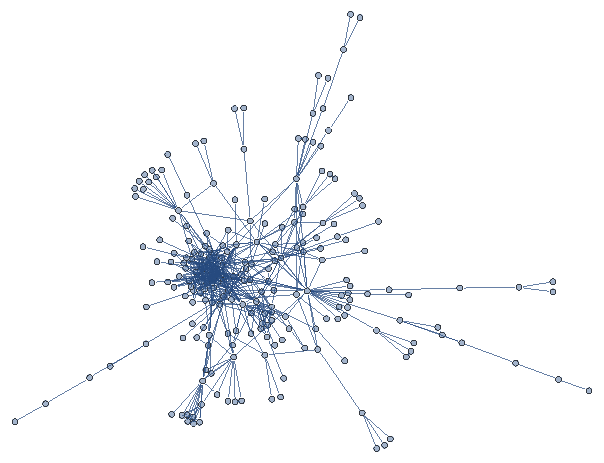
\includegraphics[width=5cm,height=4cm,angle=90]{\networksfigsdir/graph_standard.pdf}
    };
  \end{scope}
  \begin{scope}[xshift=4.5cm]
    \node [mybox] (box){
      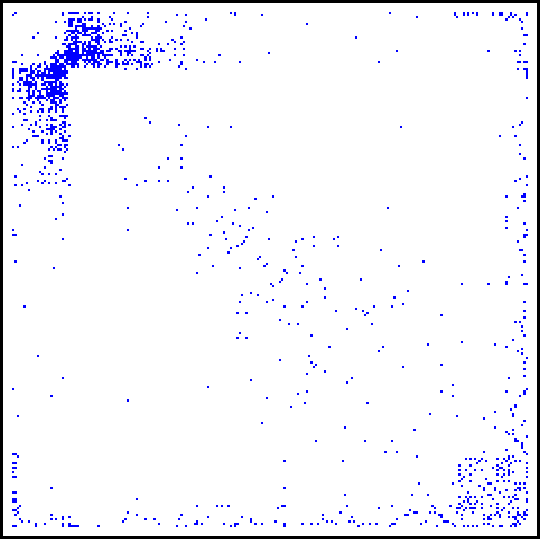
\includegraphics[width=3.5cm]{\networksfigsdir/interactome_adjacency_mathematica.pdf}

  };
  \end{scope}  
  \begin{scope}[xshift=9.2cm]
    \node [mybox] (box){
      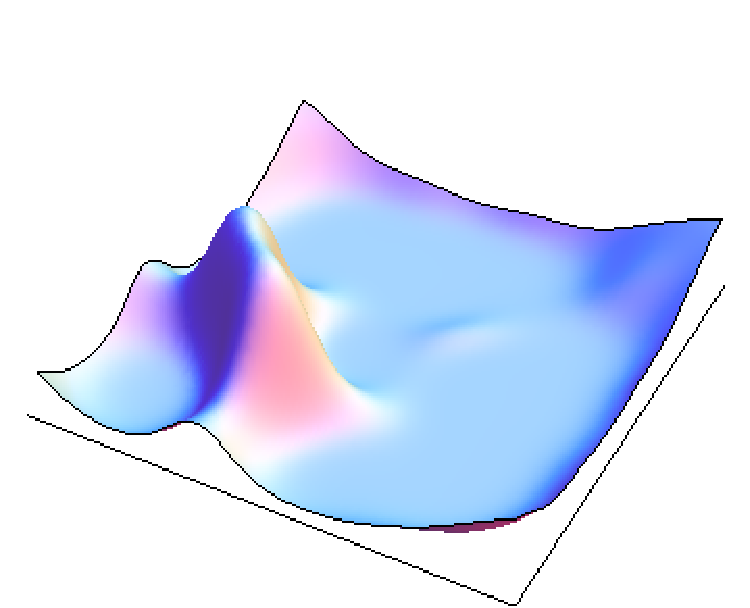
\includegraphics[width=5cm]{\networksfigsdir/graphon_listplot_bmp.pdf}
  };
  \end{scope}
\end{tikzpicture}
